\documentclass[a4paper,11pt]{article}%必须以此为开头,可以在[]内设置栏数,单双面,横竖向
\usepackage{latexsym}%符号字体
\usepackage{makeidx}%制作索引
\makeindex
\usepackage{ifthen}%提供分支语句
\usepackage{ctex}%提供中文支持
\usepackage{graphicx}%用于插入图片
\usepackage{amsmath}%用于数学公式
\usepackage{IEEEtrantools}%用于使用IEEE数学公式排版工具
\usepackage{amsfonts}%用于其他字体的数学符号
\usepackage{amsthm}%提供证明,定理等环境
\usepackage{amssymb}%用于提供各种数学符号
\usepackage{mathrsfs}%用于提供花体字母
\usepackage{verbatim}%使用\verbatiminput{filename}来直接导入文件中的文本内容
\usepackage{layouts}%用于设置页面布局
\usepackage{calc}%允许一些常量参量用算术表达式代替
\usepackage{hyperref}
\usepackage{makecell}%允许表格的单元格内换行
\usepackage{bm}%使用bm来对希腊字母加粗
\usepackage{longtable}
\usepackage{slashed}
\theoremstyle{remark}
\newtheorem*{remark}{注}
\theoremstyle{remark}
\newtheorem*{example}{例}
\theoremstyle{definition}
\newtheorem{theorem}{定理}[section]
\theoremstyle{definition}
\newtheorem*{definition}{定义}
\theoremstyle{definition}
\newtheorem{corollary}{引理}[section]
\newcommand*{\abs}[1]{\lvert #1 \rvert}
%伪代码
\usepackage{algorithm}
\usepackage{algorithmicx}
\usepackage{algpseudocode}
\usepackage{amsmath}
%伪代码
%代码块
\usepackage{ listings}
\usepackage[x11names]{xcolor}
\definecolor{mygreen}{rgb}{0,0.6,0}
\definecolor{mygray}{rgb}{0.5,0.5,0.5}
\definecolor{mymauve}{rgb}{0.58,0,0.82}
\lstset{ %
	backgroundcolor=\color{white},      % choose the background color
	basicstyle=\footnotesize\ttfamily,  % size of fonts used for the code
	columns=fullflexible,
	tabsize=4,
	breaklines=true,               % automatic line breaking only at whitespace
	captionpos=b,                  % sets the caption-position to bottom
	commentstyle=\color{mygreen},  % comment style
	escapeinside={\%*}{*)},        % if you want to add LaTeX within your code
	keywordstyle=\color{blue},     % keyword style
	stringstyle=\color{mymauve}\ttfamily,  % string literal style
	frame=single,
	rulesepcolor=\color{red!20!green!20!blue!20},
	% identifierstyle=\color{red},
	language=c,
}
%代码块
%引用
\usepackage{framed}
\usepackage{quoting}
 \colorlet{shadecolor}{Turquoise1!20}
\newenvironment{shadedquotation}
 {\begin{shaded*}
  \quoting[leftmargin=0pt, vskip=0pt]
 }
 {\endquoting
 \end{shaded*}
}
%引用
%跨页伪代码
\makeatletter
\newenvironment{breakablealgorithm}
  {% \begin{breakablealgorithm}
   \begin{center}
     \refstepcounter{algorithm}% New algorithm
     \hrule height.8pt depth0pt \kern2pt% \@fs@pre for \@fs@ruled
     \renewcommand{\caption}[2][\relax]{% Make a new \caption
       {\raggedright\textbf{\ALG@name~\thealgorithm} ##2\par}%
       \ifx\relax##1\relax % #1 is \relax
         \addcontentsline{loa}{algorithm}{\protect\numberline{\thealgorithm}##2}%
       \else % #1 is not \relax
         \addcontentsline{loa}{algorithm}{\protect\numberline{\thealgorithm}##1}%
       \fi
       \kern2pt\hrule\kern2pt
     }
  }{% \end{breakablealgorithm}
     \kern2pt\hrule\relax% \@fs@post for \@fs@ruled
   \end{center}
  }
\makeatother
%跨页伪代码
\floatname{algorithm}{算法}
\renewcommand{\algorithmicrequire}{\textbf{输入:}}
\renewcommand{\algorithmicensure}{\textbf{输出:}}
\author{范潇}
\title{ID3算法实现实验报告}
\date{2023年12月5日}
\begin{document}
\lstset{breaklines}%这条命令可以让LaTeX自动将长的代码行换行排版
		\lstset{extendedchars=false}%这一条命令可以解决代码跨页时,章节标题,页眉等汉字不显
		%示的问题
		\lstset{numbers=left,numberstyle=\tiny,keywordstyle=\color{blue!70},
			commentstyle=\color{red!50!green!50!blue!50},frame=shadowbox,
			rulesepcolor=\color{red!20!green!20!blue!20},escapeinside=``,
			%xleftmargin=-10em,xrightmargin=-23em,
            aboveskip=1em} 
\pagestyle{plain}
\maketitle
\section{实验目的}
\begin{enumerate}
    \item 掌握决策树算法(ID3)的基本思想
    \item 掌握决策树算法实现的细节
    \item 熟悉算法测试的基本流程
\end{enumerate}
\section{实验内容}
\begin{enumerate}
    \item 利用C++语言编写决策树算法(ID3)
    \item 选取适当的数据集
    \item 对选取的数据集进行预处理及划分
    \item 利用验证集选取最佳的超参数
    \item 对编写的算法进行5折交叉验证
\end{enumerate}
\section{实验过程}
\subsection{程序编写}
整个算法的具体实现分为5个部分:
\begin{enumerate}
    \item 用于存储数据集的数据结构设计
    \item 用于存储决策树的数据结构设计
    \item csv文件读取函数
    \item 决策树构造函数
    \item 用于测试和打印结点信息的函数
\end{enumerate}
\subsubsection{用于存储数据集的数据结构设计}
由于在构造决策树的递归过程中,用于决策的样本个数以及属性在不断减少,所以需要一个能够灵活变化的数据结构来存储输入的数据集。
因为在C++中没有python的pandas库中所提供的DataFrame数据结构,所以需要自行设计所需的数据结构。
\begin{lstlisting}[language={[ANSI]C},keywordstyle=\color{blue!70},commentstyle=\color{red!50!green!50!blue!50},frame=shadowbox,
    rulesepcolor=\color{red!20!green!20!blue!20}]
//用于存储数据集的相关数据结构
typedef enum {
	CON = 0,//连续型
	DIS,//离散型
	CLASS,//类别
}data_type;
typedef vector<double> dis_data;//存储离散型数据
typedef struct {//存储连续型数据
	vector<double> raw_data;//原始数据
	double sep;//连续型数据离散化后所得的分界点
}con_data;
typedef pair<con_data, dis_data>  my_data;
typedef struct {//一列数据
	data_type type;//数据类型 
	my_data data;//该列数据
}my_column;
class dataset {//数据集
private:
	vector<string> header;
	vector<my_column> column;
	int attr_num;//属性个数
	int data_num;//样本个数
	double entropy;//熵
	int class_col;//类别所在列
public:
//未列出成员函数
};
\end{lstlisting}
其中,数值型数据离散化的伪代码如下:
\begin{breakablealgorithm}
    \caption{数值型数据离散化}
    \begin{algorithmic}[1]
        \Require 待离散化的一列数值型数据data
        \Ensure 分界点sep
        \Function {discritization}{vector$<$double$>$\,data}
        \State 将data中的数据按照升序存储进辅助数组temp中
        \State 将temp中每组相邻元素的平均数依次存放进辅助数组candidate中
        \State 将candidate中的元素依次取出,并计算以此为分界点时所得到的两个子数据集的熵值之和
        \State \Return 使得熵值之和最小的元素
        \EndFunction
    \end{algorithmic}
\end{breakablealgorithm}
\subsubsection{用于存储决策树的数据结构设计}
\begin{lstlisting}[language={[ANSI]C},keywordstyle=\color{blue!70},commentstyle=\color{red!50!green!50!blue!50},frame=shadowbox,
    rulesepcolor=\color{red!20!green!20!blue!20}]
//决策树结点
struct DT {
	data_type type;//存储的数据类型
	double sep;//存储连续型属性的分界点
	vector<double> val;//存储离散型属性的可能取值
	string header;//属性名称
	int ch_num;//孩子节点个数
	DT** children;//孩子结点数组
	double result;//存储的是叶子结点中的类别
	double entropy;//熵
	int data_num;//样本个数
};
//决策树
class DecisionTree {
public:
	DT* DTree;
	DecisionTree();
	void construct(DT*& root,dataset& source,double result_for_empty_data,int first);
	void test(dataset& test_set);
	void print(DT*,int );
	friend dataset;
};
\end{lstlisting}
\subsubsection{csv文件读取函数}
该函数要求用户依次输入训练集和测试集的文件名,然后输入阈值,最后会分别打印出训练集和测试集中各列的标题,
并要求用户对每一列的数据进行分类。由于ID3决策树算法在处理连续型属性之前,需要先将其离散化,因此要求用户把数值属性用“C”标记出来。
同时,要求用户把标称属性、类别、不参与决策树构造的属性分别用“D”、“T”、“X”标记出来。

\subsection{决策树构造函数}
\begin{breakablealgorithm}
    \caption{ID3算法构造决策树}
    \begin{algorithmic}[1]
        \Require 根节点root,数据集source
        \Function {construct}{DT*\&\,root,dataset\&\,source}
        \If{source中无样本}
        \State{root$\rightarrow$children =NULL}
        \State{root$\rightarrow$result置为原始数据集中类别占比最多的一类}
        \Else\If{source中无属性}
        \State{root$\rightarrow$children =NULL}
        \State{root$\rightarrow$result置为当前数据集中类别占比最多的一类}
        \Else
         \State {求最大信息增益}
        \If{不超过阈值}
        \State{root$\rightarrow$children =NULL}
        \State{root$\rightarrow$result置为当前数据集中类别占比最多的一类}
        \Else 
        \State{将当前数据集按照信息增益最多的那个属性进行划分,然后递归}
        \EndIf
        \EndIf
        \EndIf
        \EndFunction
    \end{algorithmic}
\end{breakablealgorithm}
\subsection{用于测试和打印结点信息的函数}
测试函数要求的输入是测试集。对于测试集中的每一个样本,它将按照其属性值,在已经构造好的决策树中搜索叶子结点,并将得到的值与测试集中对应样本的类别进行比较。

打印结点的函数采用的是横向打印,对于每个非叶子结点,将会输出对应数据表的熵、其中的样本数、以及能使信息增益最大的属性的信息。对于叶子节点,则会打印其对应的类别、
样本数、以及熵。
\subsection{数据集的选择}
在挑选用于训练ID3决策树算法的数据集时,我所采用的标准是:1.数据规模较小;2.属性个数较少;3.即有标称属性,又有数值属性;4.缺失值较少。最终我选用了Kaggle平台上的Obesity Classification数据集。
\subsection{数据集预处理和划分}
我将“ID”这一列数据删去,并将“Gender”和“Label”这两列标称数据进行独热编码,其中“偏瘦”、“正常”、“偏胖”、“肥胖”分别被编码为0、1、2、3。
然后将该数据集按照8:2的比例划分为训练集和验证集,最后再将它按照5折交叉验证的要求进行划分。
\subsection{超参数的选取}
\begin{figure}[htbp]
    \centering
    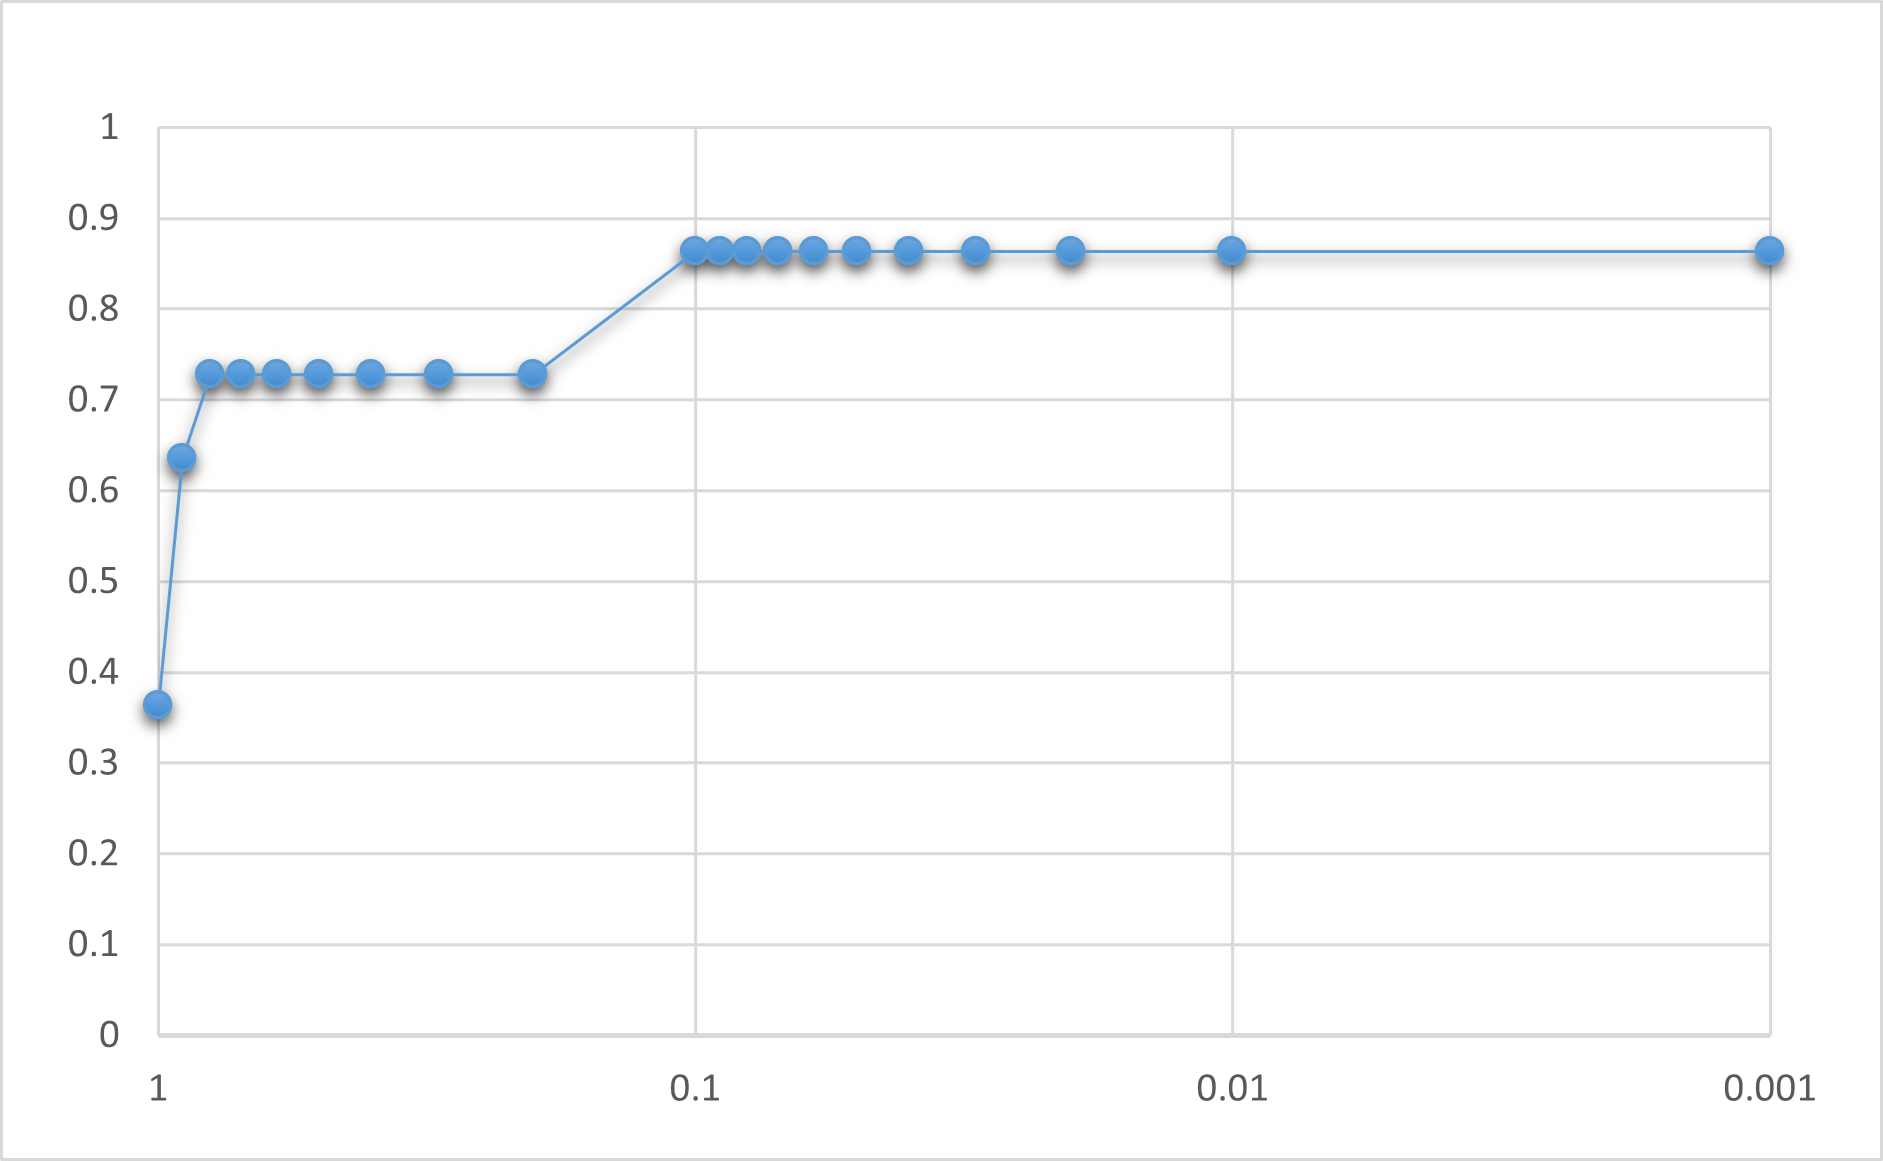
\includegraphics[scale=0.7]{pic.png}
    \caption{超参数与准确率的关系}
\end{figure}
经过测试,最终将超参数选取为0.05.
\section{测试样例说明}
原数据集共有108份样例,有“ID”、“Age”、“Gender”、“Height”、\\
“Weight”、“BMI”、“Label”六列数据。
其中“ID”不参与决策树的构造,“Age”、“Gender”、“Height”、“Weight”、“BMI”为数值型数据,\\
“Gender”、“Label”为标称型数据。
“Label”即肥胖程度,是该数据集中的样本的类别,总有4类:“Underweight”、“Normal Weight”、“Over-\\
weight”、“Obese”。
\begin{figure}[htbp]
    \centering
    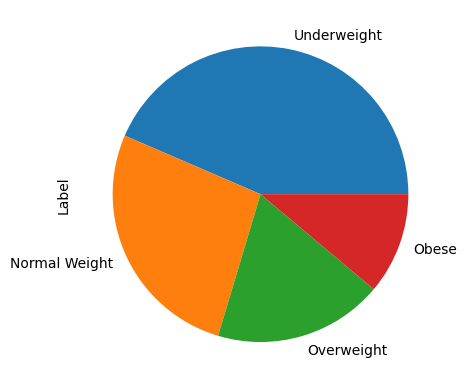
\includegraphics[scale=0.8]{output.png}
    \caption{Label的分布情况}
\end{figure}
\section{测试结果及分析}
经过调参后,程序在验证集上的最高准确率达到86.3636\%。当超参数,即阈值,选为0.05时,在5折交叉验证中的准确率分别为86.3636\%、
68.1818\%、90.9091\%、85.7143\%、71.4286\%,平均准确率为80.5195\%。
\begin{figure}[htbp]
    \centering
    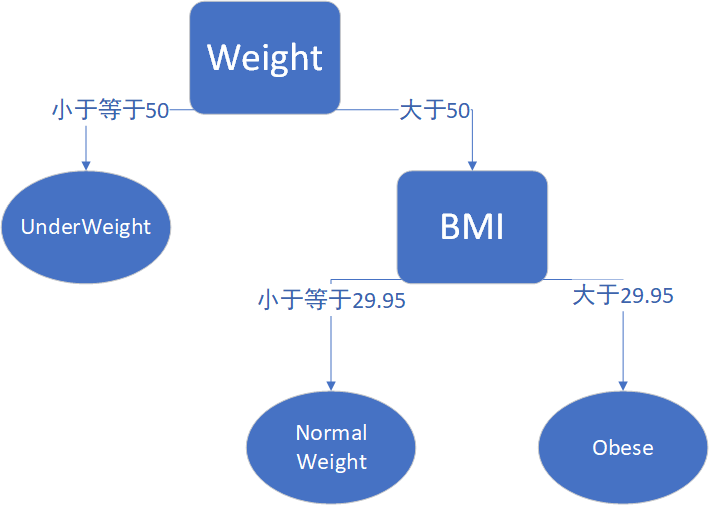
\includegraphics[scale=0.425]{tree.png}
    \caption{算法生成的决策树}
\end{figure}

以准确率为90.9091\%的实验中生产的决策树为例,根据该决策树最多只需进行两次判断即可结束分类,第一次根据体重进行分类,如果相对较轻,则分类为
“Underweight”,否则继续比较BMI。如果BMI又较大,则分为“Obese”,否则分为”Normal Weight”。这两次比较的依据都十分符合常识,因为医学上判断是否肥胖
的指标无外乎体重和BMI。之所以该决策树并没有“Overweight”对应的叶子结点,是因为没有达到相应的阈值。而在这种情况下仍能够达到较高的准确率的原因之一是
测试集样本的分布不均匀:在该测试集中,只有一个“Overweight”的样本。但是由于使用了K折交叉验证,由于测试集中样本的分布而导致的误差已被抵消掉一部分了。
\end{document}